\section{Clase 19}
\subsection{Expansión del Virial}
Teníamos 
\begin{equation}\label{19.VdW}
  P=\frac{\r\k T}{1-\r/\r_s}-a\r^2
\end{equation}
donde $\r_s=1/$ son parámetros fenomenológicos (interpretación de aproximación de campo medio).

Las ecuaciones de estado pueden escribirse como una exresión de la densisdad numérica (\textit{expansión del virial}) de la forma
\begin{equation}\label{19.virial}
  P=\r\k T\left[A_1+\sum_{n=2}^\infty A_n\left(\frac{\r }{\r_0}\right)^{n-1}\right]
\end{equation}
con
\begin{equation}
  \r_0=\frac{2s+1}{(2\p\hbar)^3}\int\dd^3 pe^{-\epsilon(p)/\k T}
\end{equation}
la densidad del gas ideal.

\begin{ej}
	Encontremos la expansión del virial par el ags de Van der Waals.
\end{ej}

\begin{sol}
	Recordemos la serie geométrica
	\begin{equation}
  \sum_{i=0}^\infty x^{i}=\frac{1}{1-x},\qquad |x|<1
\end{equation}
Luego, de \eqref{19.VdW},
\begin{align}
  P&=\frac{\r\k T}{1-\r/\r_s}-a\r^2\\
  &=\r\k T\left(\frac{1}{1-\r/\r_s}\right)-a\r^2\\
  &=\r\k T\left(\sum_{i=0}^\infty\left(\frac{\r }{\r_s}\right)^{i}\right)-a\r^2\\
  &=\r\k T\left(1+\frac{\r}{\r_s}+\sum_{i=2}^\infty\left(\frac{\r }{\r_s}\right)^{i}x\right)-a\r^2
\end{align}
comparando coeficiente entre potencias de $\r$ con \eqref{19.virial}, es directo ver que
\begin{align}
  A_1&=1\\
  A_2&=\frac{\r_0}{\r_s}-\frac{a\r_0}{\k T}\\
  A_{i>3}&=\left(\frac{\r_0}{\r_s}\right)^{i-1}
\end{align}
\end{sol}

Usando la ecuación de estado podemos encontrar la energía por partícula para el fluido. Para hacer esto consideremos la siguiente relación de Maxwell
\begin{equation}
\eval{  \pdv{(P/\k T)}{\b}}_{N,V}=-\eval{\pdv{E}{V}}_{N,T}
\end{equation}
Queremos encontrar $\frac{E}{N}(\r )$. De \eqref{19.VdW},
\begin{equation}
  \frac{P}{\k T}=\frac{\r }{1-\r/\r_s}-\b a\r^2
\end{equation}
\begin{equation}
  \implies \pdv{\b}\left(\frac{P}{\k T}\right)=\pdv{\b}\left(\frac{\r }{1-\r/\r_s}-\b a\r^2\right)=-a\r^2
\end{equation}
Considerando que a $\r\approx 0$ el fluido se comporta como un gas ideal, se tiene a siguiente condición de borde
\begin{equation}\label{19.borde}
  \frac{E}{N}(\r=0)=\frac{3}{2}\k T
\end{equation}
Necesaitamos la derivada con respecto a $\r$, así que cambiamos los diferenciales,
\begin{equation}
  V=\frac{N}{\r }\implies \eval{\pdv{V}}_N=-\frac{\r^2}{N}\eval{\pdv{\r}}_N
\end{equation}
luego, 
\begin{equation}
  \pdv{E}{\r }=-aN
\end{equation}
Luego, tenemos la siguiente ecuación diferencial sujeta a la condición inicial \eqref{19.borde}. Dado que $E/N$ no depende de $N$ ni $T$, podemos escribir,
\begin{equation}
  \dv{(E/N)}{\r }=-a
\end{equation}
\begin{equation}
  \implies \eval{\frac{E}{N}}_{\r=0}^{\r=\r }=-\eval{a\r }_{\r=0}^{\r=\r }
\end{equation}
\begin{equation}
\boxed{  \frac{E}{N}(\r )=-a\r +\frac{3}{2}\k T}
\end{equation}
Luego, vemos que por la energía promedio por partícula es menor de lo que sería para el gas ideal. Esto se entiende como efecto del término de atracción.

\subsection{Coexistencia entre fase líquida y gaseosa}
La función $P(V)$ \textit{no} es monótona en general. En efecto, para
\begin{equation}
  T<T_c=\frac{8a\r_s}{27\k }
\end{equation}
la curva tiene un mínimo.

El régimen $(\pdv*{P}{V})_T>0$ \textit{no es físico} (un fluido cuya presión disminuye al aumentar el volumen no es estable, pues tendería a comprimirse espontáneamente). En realidad, cuando en una curva isoterma se tiene $(\pdv*{P}{V})_T>0$, lo que sucede es que la \textit{presencia de diferentes fases o estados de la materia coexisten}.

\subsection{Coexistencia de fases}
\begin{figure}[h!]
	\centering
	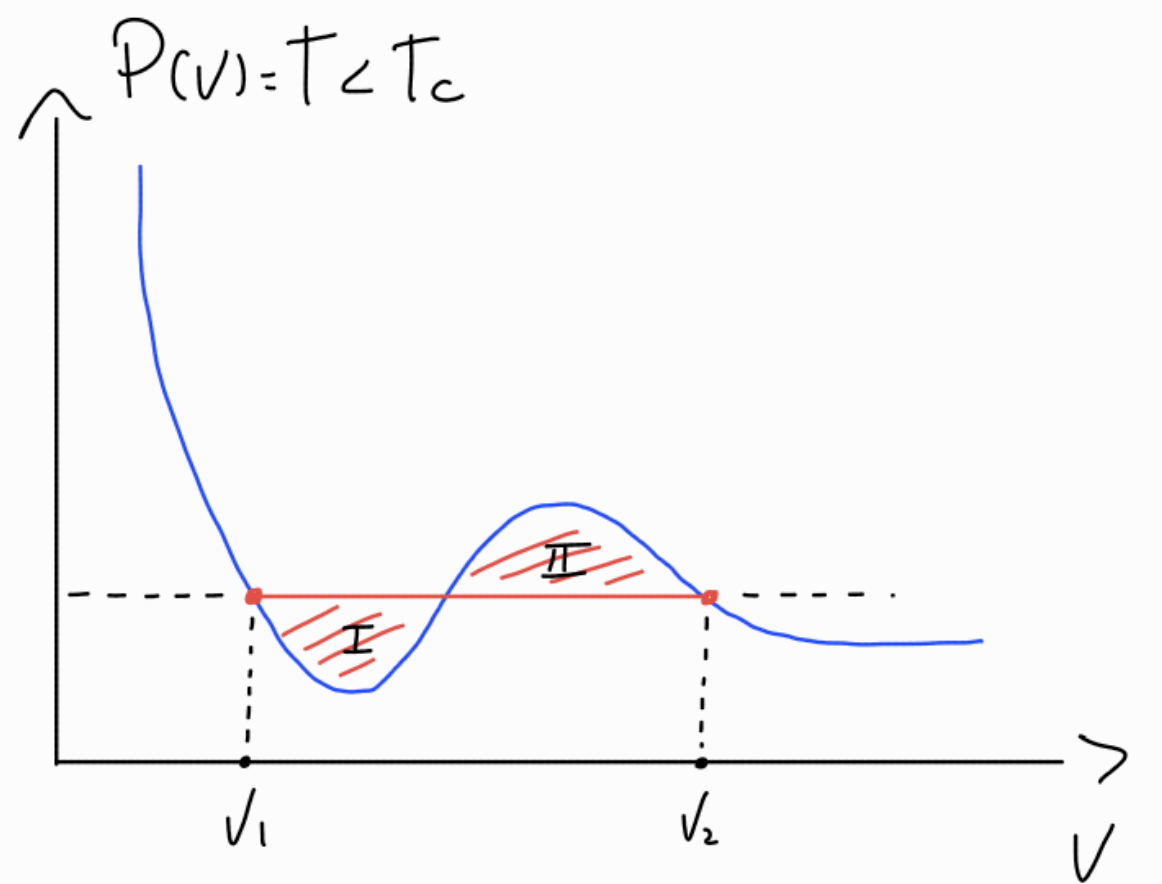
\includegraphics[scale=0.4]{fig/18.png}
\end{figure}

De acuerdo con la construcción de áreas iguales de Maxwell, la verdadera isoterma $P(V)$ del fluido sigue la curva de la ecuación de estado para $V<V_1$ y para $V>V_2$, pero es una línea recta horizontal ($P=$ constante) para $V$ entre $V_1$ y $V_2$.

El valor de $V_1$ y $V_2$ está determinado de forma que el área $I$ sea igual al área $II$ en el diagrama $PV$.

La compresión entre $V_2$ y $V_1$ es isobárica y lo que sucede es que el fluido se convierte progresivamente de gas a liquido hasta llegar al volumen $V_1$.
\begin{itemize}
	\item Para $V<V_1$, todo el fluido está en fase líquida.
	\item  Para $V>V_2$, todo el fluido está en fase gaseosa.
\end{itemize}










